\documentclass[runningheads,a4paper]{llncs}
\usepackage{color}
\usepackage{amssymb}
\setcounter{tocdepth}{3}
\usepackage{graphicx}
\usepackage{framed}
\usepackage{url}
\urldef{\mailsa}\path|firstname.lastname@gesis.org|
\newcommand{\keywords}[1]{\par\addvspace\baselineskip
\noindent\keywordname\enspace\ignorespaces#1}

\begin{document}

\mainmatter  % start of an individual contribution

% first the title is needed
\title{Analyzing the research output presented at European Networked Knowledge Organization Systems workshops (2000-2015)}

% a short form should be given in case it is too long for the running head


% the name(s) of the author(s) follow(s) next
%
% NB: Chinese authors should write their first names(s) in front of
% their surnames. This ensures that the names appear correctly in
% the running heads and the author index.
%
\author{Fakhri Momeni%
	\and Philipp Mayr}
%
\titlerunning{Analyzing the NKOS research output (2000-2015)}
% (feature abused for this document to repeat the title also on left hand pages)

% the affiliations are given next; don't give your e-mail address
% unless you accept that it will be published
\author{Fakhri Momeni and Philipp Mayr}
\institute{GESIS - Leibniz Institute for the Social Sciences,\\
	Unter Sachsenhausen 6-8\\
	50667 Cologne, Germany\\
	\email{firstname.lastname@gesis.org} }

%
% NB: a more complex sample for affiliations and the mapping to the
% corresponding authors can be found in the file "llncs.dem"
% (search for the string "\mainmatter" where a contribution starts).
% "llncs.dem" accompanies the document class "llncs.cls".
%

%\toctitle{Lecture Notes in Computer Science}
%\tocauthor{Authors' Instructions}
\maketitle


\begin{abstract}		
In this paper we analyse a major part of the research output of the Networked Knowledge Organization Systems (NKOS) community in the period 2000 to 2015. We focus on the paper output presented at the European NKOS workshops in the last 15 years. Our open dataset "the NKOS bibliography" includes 14 workshop programmes (ECDL 2000-2010, TPDL 2011-2015) and 4 special  issues on NKOS (2001, 2004, 2006 and 2015) which cover in total n %add number
papers with n %add number
single authors. A focus of the analysis is the development of collaboration, core authors and topics in this interdisciplinary field. %be more precise

%add some more facts
 
\keywords{NKOS workshops, Special issues, Output analysis, Network analysis, Central authors, Collaboration}
\end{abstract}


\section{Introduction}\label{intro}
%intro and motivation %philipp

The European NKOS network has held a long-running series of annual workshops at the European Conference on Digital Libraries (ECDL), latterly reformed as the International Conference on Theory and Practice of Digital Libraries (TPDL). 
Typically, recent advances of KOS have been reported at the NKOS workshops, e.g. including the Simple Knowledge Organization System (SKOS) W3C standard, the ISO 25964 thesauri standard, the CIDOC Conceptual Reference Model (CRM), Linked Data applications, KOS-based recommender systems, KOS mapping techniques, KOS registries and metadata, social tagging, user-centred issues, and many other topics. A comprehensive and well cited review article on KOS was published in 2004 \cite{Zeng2004}. Special issues on Networked Knowledge Organization Systems (NKOS) have been published in Journal of Digital Information in 2001 and 2004, in New Review of Hypermedia and Multimedia in 2006 and in the International Journal of Digital Libraries in 2015 \cite{Mayr2016}. 

The motivation of this paper is to analyse the research output of the NKOS community. We are focusing on the informal part of this output, the presentations given the workshops. The specialty of this output is that these research papers typically are not published in journals or conference proceedings, these papers appear just as oral presentations at the workshop and are documented on the website. To our knowledge nobody has done an analysis on this part of the research output before. 



\section{NKOS workshop bibliography}\label{dataset}
%data set description %philipp

For our analysis we have compiled an open dataset the "NKOS bibliography"\footnote{The NKOS workshop bibliography is maintained in the following github repository: https://github.com/PhilippMayr/NKOS-bibliography} which includes 14 workshop programmes with all presented papers at ECDL 2000, 2003-2010 and TPDL 2011-2015. We added papers from 4 special issues on NKOS which have been published in the same period.

In a first step we have extracted all paper titles presented at the NKOS workshop websites. We manually disambiguated author names. We added the papers from the special issues. These paper are the only formal publications in our analysis.

Our dataset covers in total n %add number
papers with n %add number
single authors.

Table provides an overview of all workshop papers.

%include an overview table (venue;# of papers;# of authors; av # of authors)

\begin{tabular}	{|c|c|c|}
	\hline 
	venue& papers  & authors  \\ 
	\hline 
	ECDL 2000&  &  \\ 
	\hline 
	ECDL 2003&  &  \\ 
	\hline 
	ECDL 2004&  &  \\ 
	\hline 
	ECDL 2005&  &  \\ 
	\hline 
	ECDL 2006&  &  \\ 
	\hline 
	ECDL 2007&  &  \\ 
	\hline 
	ECDL 2008&  &  \\ 
	\hline 
	ECDL 2009&  &  \\ 
	\hline 
	ECDL 2010&  &  \\ 
	\hline 
	TPDL 2011&  &  \\ 
	\hline 
	TPDL 2012&  &  \\ 
	\hline 
	TPDL 2013&  &  \\ 
	\hline 
	TPDL 2014&  &  \\ 
	\hline 
	TPDL 2015&  &  \\ 
	\hline 
\end{tabular} 


Table provides an overview of all papers in the special issues.

\begin{tabular}{|c|c|c|}
	\hline 
	venue& papers  & authors  \\ 
	\hline 
	SI 2001&  &  \\ 
	\hline 
	ECDL 2004&  &  \\ 
	\hline 
	ECDL 2006&  &  \\ 
	\hline 
	ECDL 2015&  &  \\ 
	\hline 
\end{tabular} 


%The most cited NKOS papers in this time: Zeng, Dörr ... Koch 



\section{Analysis}\label{analysis}
Description of the types of analyses %fakhri

\section{Results}\label{results}
Describing the results %fakhri



\begin{figure}
\centering
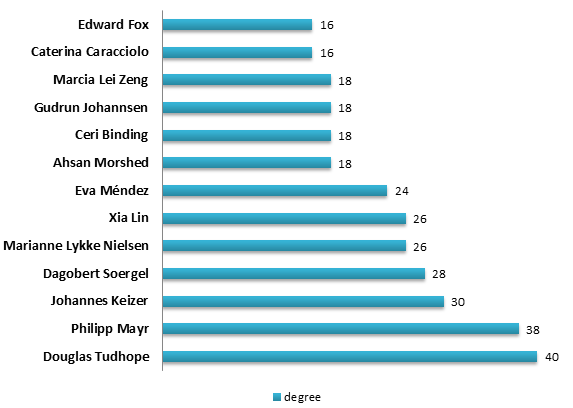
\includegraphics[width=0.7\linewidth]{degree16}
\caption{}
\label{fig:degree16}
\end{figure}

...

\begin{figure}
\centering
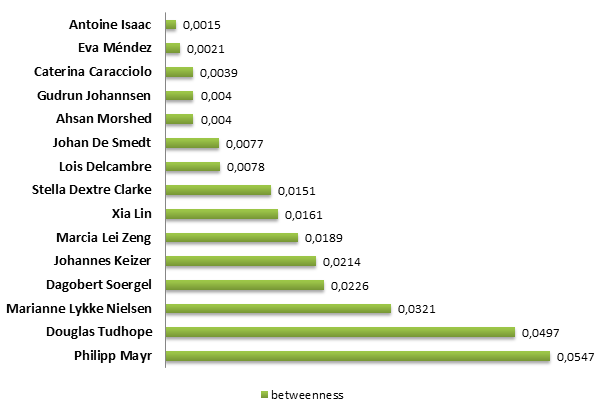
\includegraphics[width=0.7\linewidth]{betweenness}
\caption{}
\label{fig:betweenness}
\end{figure}

...

\begin{figure}
\centering
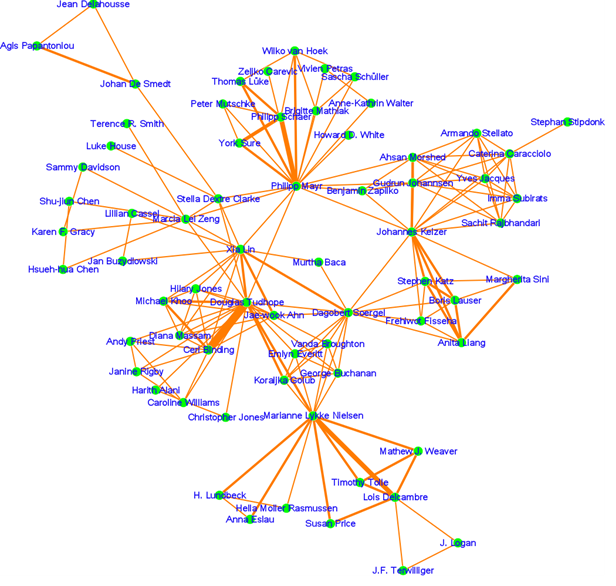
\includegraphics[width=0.7\linewidth]{network}
\caption{}
\label{fig:network}
\end{figure}



\section{Conclusion}\label{concl}
...%both

\section{Acknowledgment}\label{sec:ACKNOWLEDGMENTS}
...

\newpage

\bibliographystyle{splncs03} % abbrev
\bibliography{nkos} 

\end{document}
